\section{Randomness and Shuffling}
In the game of poker, the house does not wager against players, unlike other 
popular casino games, such as blackjack or roulette, but instead the usual 
method for online poker companies and indeed poker tables in real life to make 
money is the rake. 

The implementation of the rake varies between casinos and online poker
software. Some common ones are in the below table.

\begin{center}
    \begin{tabular}{l l}
    \toprule
    Mechanism           & Description                                               \\
    \midrule
    Pot Rake            & Percentage taken from the pot, per hand or betting round  \\ \addlinespace
    Dead Drop           & Fee paid by the player with the dealer button each hand   \\ \addlinespace
    Timed Rake          & Set fee collected every set interval of time              \\ \addlinespace
    Fixed Fee           & Fixed fee per hand                                        \\ \addlinespace
    Tournament Fee      & Entry fee to participate in poker tournaments             \\ \addlinespace
    Subscription Fees   & Players are charged a subscription fee to play            \\
    \bottomrule
    \end{tabular}
\end{center}

Finally, some games are rake free, instead generating revenue by driving
traffic to more profitable businesses. The software developed that this paper
is discussing is also rake free, due to being only for academic purposes.

However, despite companies being able to generate revenue in these ways, the
implementation of random number generation in poker software is a topic of
some interest. Possible issues include rogue employees writing malicious
code to give them or people connected to them beneficial cards, faulty code
allowing the random number generation to be exploited, and other schemes, such
as giving newer players or failing players better cards, to encourage them to 
continue using the companies platform, and generating revenue through rakes.

For these reasons, random number generation has been analysed and multiple
different shuffling algorithms or card picking algorithms have been
developed and contrasted for possible weaknesses. Two obvious approaches to 
selecting cards are:

\begin{itemize}
    \item Storing an array of all the cards and indexing this array in some way to take a card
    \item Shuffling an array in some way and taking the top item
\end{itemize}

\newpage

Multiple versions of both these algorithms have been implemented, using
different sources of randomness. Also developed is a GUI which can be launched
when the `--chooseshuffle' argument is given to the server, which allows
the card picking algorithm and random source to be altered mid game. 

\begin{figure}[H]
    \centering
    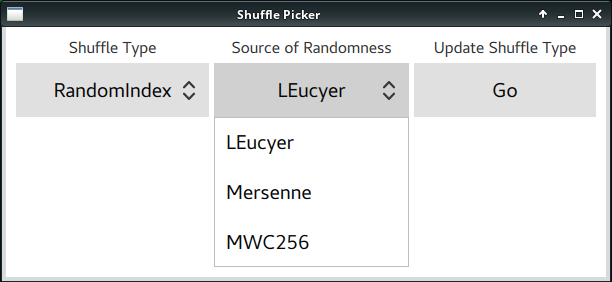
\includegraphics[width=0.8\linewidth]{../images/shufflepicker.png}
    \caption{The Shuffle Picker Window}%
    \label{fig:shufflepicker}
\end{figure}

Another program provides a similar interface but instead allows multiple hands 
to be drawn and the number of times each card was drawn displayed in a graph. 
This  allows us to easily see the effect of the different algorithms on the 
uniformness of the card distribution.

\begin{figure}[H]
    \centering
    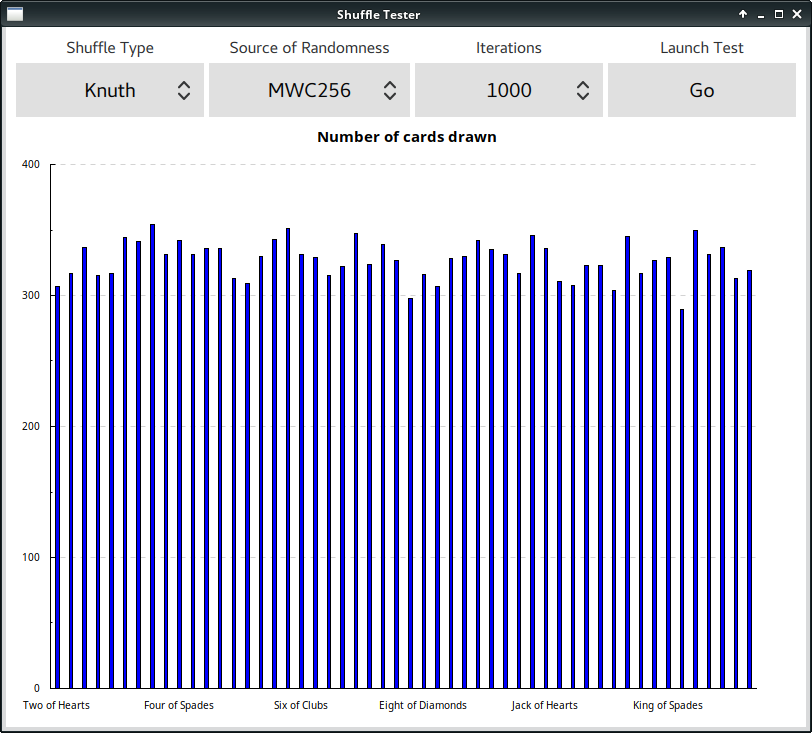
\includegraphics[width=0.8\linewidth]{../images/shuffletester.png}
    \caption{The Shuffle Tester Program}%
    \label{fig:shuffletester}
\end{figure}

The sources of randomness and their cycles can be found in the below table.

\vspace{0.7cm}

\begin{adjustbox}{center}
    \begin{tabular}{l l}
    \toprule
    Random Source                                                   & Cycle                         \\
    \midrule

    Portable Combined Generator of L'Eucyer \parencite{leucyer1988} & See equation~\ref{eq:leucyer} \\ \addlinespace

    Fast Mersenne Twister \parencite{matsumoto1998,saito2008}       & See equation~\ref{eq:twister} \\ \addlinespace

    Multiply With Carry 256 \parencite{marsaglia2003}               & See equation~\ref{eq:mwc}     \\

    \bottomrule
    \end{tabular}
\end{adjustbox}

\vspace{0.7cm}

\begin{equation} \label{eq:leucyer}
\frac{(2147483563-1)(2147483399-1)}{2}
\end{equation}

\begin{equation} \label{eq:twister}
{2}^{19937}-1
\end{equation}

\begin{equation} \label{eq:mwc}
{2}^{8222}
\end{equation}
